\newcommand*{\hmm}{Hidden Markov Models}%
\subsection{\hmm{}}
\subsubsection{Εισαγωγή}
Ένα \hmm{} είναι μια διπλά στοχαστική διαδικασία:
υπάρχει μια κρυφή διαδικασία η οποία μπορεί να παρατηρηθεί μέσω άλλων στοχαστικών διαδικασιών που παράγουν την ακολουθία των παρατηρηθέντων συμβόλων \cite{rabiner1986introduction}.
Πρόκειται για μια Μαρκοβιανή αλυσίδα (Markov Model ή Markov Chain) με κρυφές καταστάσεις.

\begin{wrapfigure}[15]{r}{0.5\textwidth}
        \centering
        \vspace{-20pt}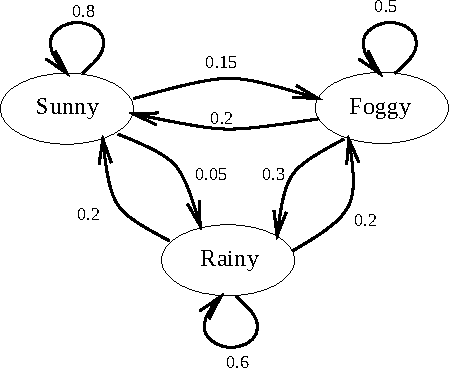
\includegraphics[width=\linewidth]{fosler1998markov-1}
        \vspace{-20pt}\caption{Παράδειγμα μαρκοβιανής αλυσίδας με υποθετικά νούμερα \protect\cite{fosler1998markov}}
        \label{fig:fosler1998markov-1}
\end{wrapfigure}

Ένα παράδειγμα Μαρκοβιανής αλυσίδας δίνεται από το \cite{fosler1998markov}:
Υποθέτουμε ότι ο καιρός έχει 3 πιθανές καταστάσεις: ηλιοφάνεια, βροχή και ομίχλη.
Χωρίζουμε τον χρόνο σε ημέρες και υποθέτουμε ότι κάθε ημέρα επικρατεί μόνο μια από τις 3 πιθανές καταστάσεις.
Θεωρούμε ότι ο καιρός της ημέρας $n$ εξαρτάται μόνο από τον καιρό της ημέρας $n-1$.
Αυτό ονομάζεται Μαρκοβιανή ιδιότητα πρώτης τάξης (first-order Markov Assumption).
Η αναπαράσταση του συστήματος αυτού φαίνεται στο \imageref{fosler1998markov-1}.

\begin{wrapfigure}[15]{r}{0.5\textwidth}
        \centering
        \vspace{-20pt}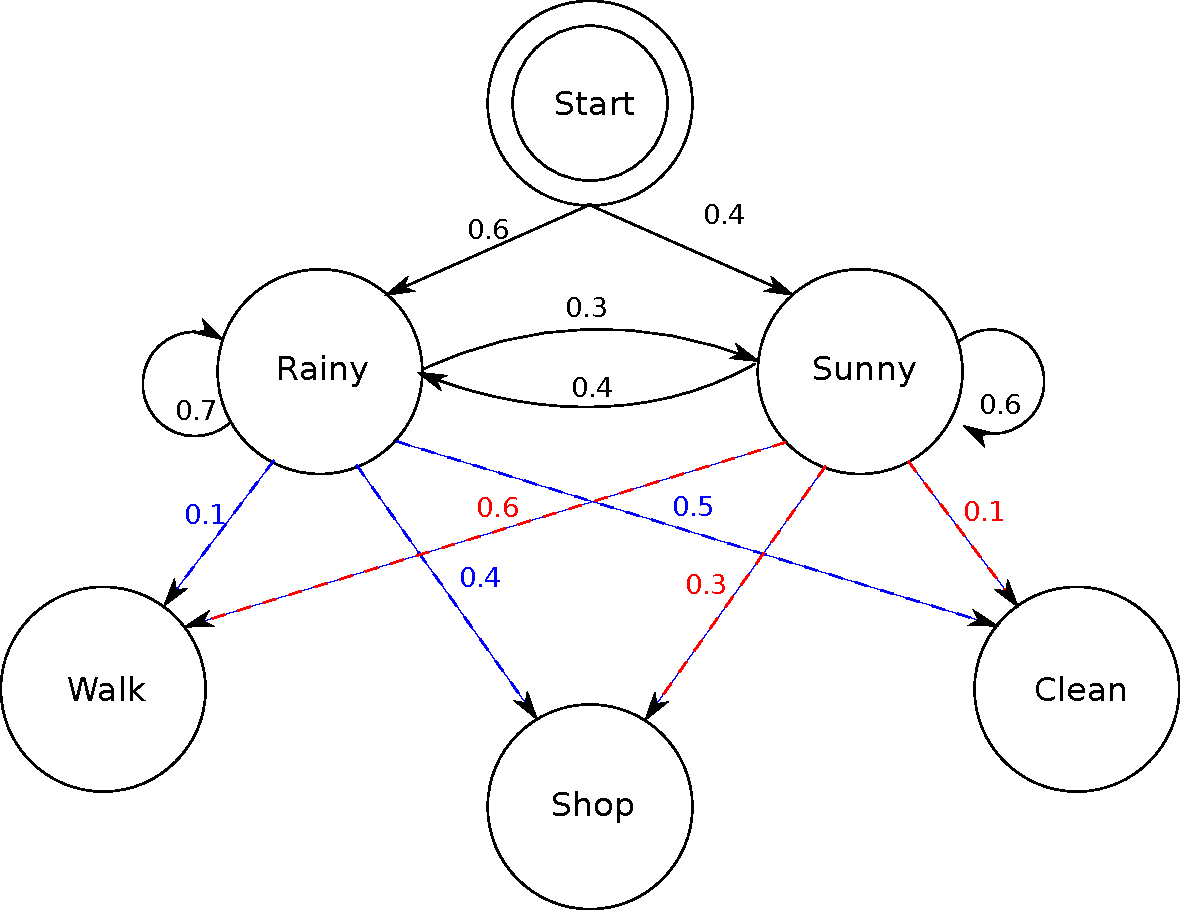
\includegraphics[width=\linewidth]{HMMGraph}
        \vspace{-20pt}\caption{Παράδειγμα κρυφής μαρκοβιανής αλυσίδας με υποθετικά νούμερα \protect\cite{wikiHMM}}
        \label{fig:HMMGraph}
\end{wrapfigure}

Αν τροποποιήσουμε το παράδειγμα έτσι ώστε να πρέπει να μαντέψουμε τον καιρό της ημέρας $n$ χωρίς να μπορούμε να παρατηρήσουμε άμεσα τον καιρό (αν είμαστε κλειδωμένοι σε ένα δωμάτιο σύμφωνα με το \cite{fosler1998markov})
αλλά έχουμε μόνο κάποιο έμμεσο τρόπο (αν αυτός που μας φέρνει το φαγητό κρατάει ομπρέλα) τότε μιλάμε για ένα \hmm{}.

Στο \imageref{HMMGraph} (από \cite{wikiHMM}) φαίνεται ένα άλλο παράδειγμα \hmm{} όπου ο παρατηρητής προσπαθεί να μαντέψει τι καιρό έχει σε ένα μέρος σύμφωνα με τις συνήθειες (Walk, Shop, Clean) του φίλου του.

\subsubsection{Εφαρμογή σε συστήματα QbSH}
\begin{figure}
    \centering
    \begin{subfigure}{0.45\linewidth}
        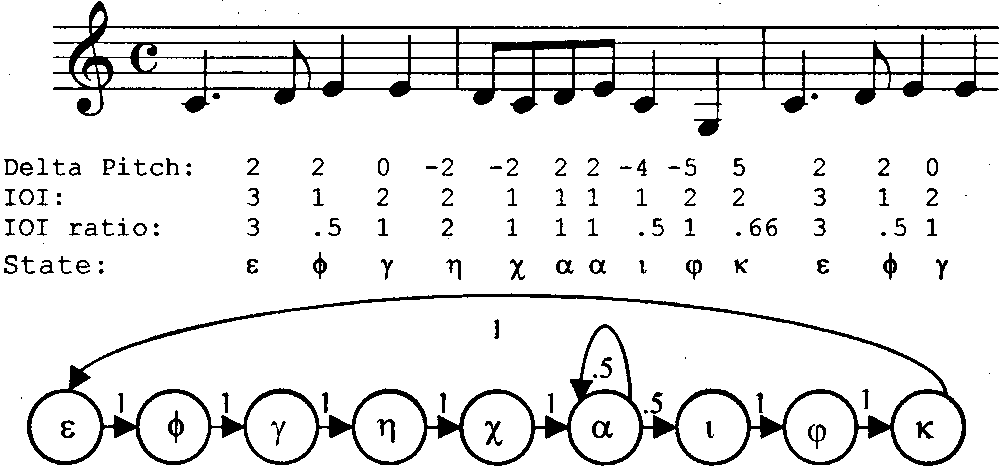
\includegraphics[height=3cm, width=\linewidth, keepaspectratio]{pardo2004name-alouette}
    \end{subfigure}\hfill
    \begin{subfigure}{0.45\linewidth}
        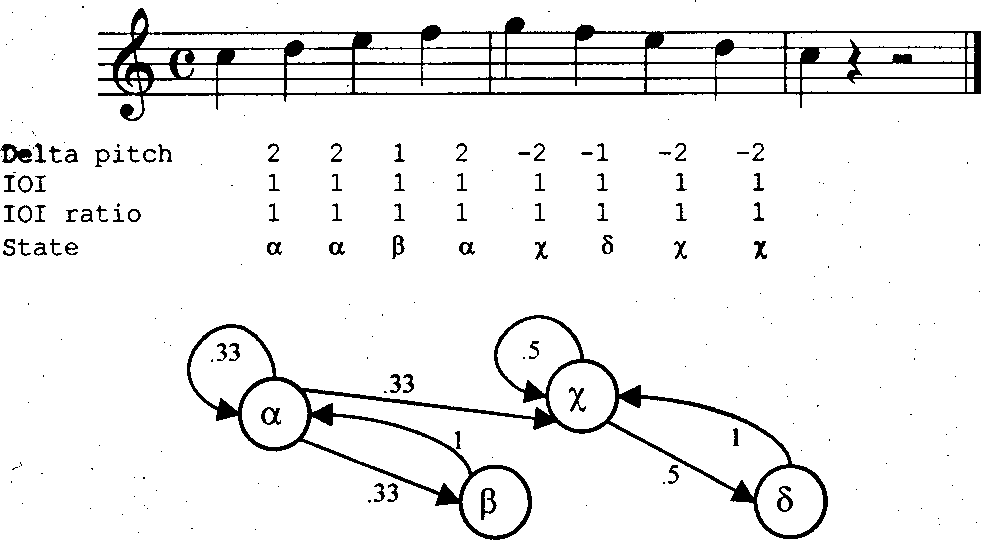
\includegraphics[height=3cm, width=\linewidth, keepaspectratio]{pardo2004name-scalar}
    \end{subfigure}
    \caption{Markov models από κομμάτια μουσικής \protect\cite{pardo2004name}}
    \label{fig:pardo2004name-alouette}
\end{figure}

Στην βιβλιογραφία υπάρχουν διάφορες αναφορές για χρήση \hmm{} σε συστήματα QbSH.
Το 2004 στο \cite{pardo2004name} περιγράφεται μια διαδικασία (\imageref{pardo2004name-alouette}) αναπαράστασης αρχείου MIDI με HMM.
Το query αναπαρίσταται σαν μια ακολουθία και ένα target θεωρείται όμοιο με το query αν το HMM που παράχθηκε από το MIDI του target έχει υψηλές πιθανότητες να δημιουργήσει την ακολουθία του query.

Στο \cite{jang2005continuous} χρησιμοποιούνται frame-based Continuous \hmm{} (CHMM) σαν υπολογιστικά καλύτερη λύση από τον \hyperref[sub:DTW]{DTW}.
Παράδειγμα δημιουργίας CHMM φαίνεται στο \imageref{jang2005continuous-chmm}.
Κάθε state στο CHMM χαρακτηρίζεται από την Gaussian probability density function (PDF):
\begin{equation*}
    g(\chi, \mu, \Sigma) = \frac{1}{\sqrt{(2\pi)^d\abs{\Sigma}}} \exp{[\frac{-(\chi-\mu)^T\Sigma^{-1}(\chi-\mu)}{2}]}
\end{equation*}
όπου $x$ είναι το $d$-διάστατο διάνυσμα παρατηρήσεων, $\mu$ και $\Sigma$ είναι τα mean vector και covariance matrix της PDF.
Για την βελτιστοποίηση των παραμέτρων των CHMM γίνεται training πάνω στο database με τα ground truth MIDI αρχεία και στις ηχογραφήσεις.

Γίνεται χρήση δυναμικού προγραμματισμού για την εύρεση της πιθανότητας ενός pitch vector να έχει παραχθεί από ένα συγκεκριμένο CHMM.
Για ένα pitch vector $x = [x_1, x_2, ..., x_m]$ και ένα CHMM με $n$ states δημιουργείται ένας $m \times n$ πίνακας $H$ δημιουργείται από τις πιθανότητες μετάβασης $p_t(i,j)$ και την $g$.
Η μέγιστη γενική πιθανότητα βρίσκεται ως $\max_{j=1...n}{H(m,j)}$.

\begin{figure}
	\centering
	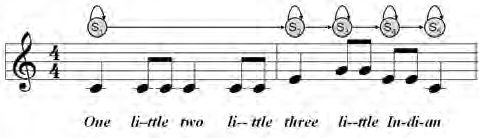
\includegraphics[width=0.65\textwidth]{jang2005continuous-chmm}
	\caption{Δημιουργία CHMM από το τραγούδι "Ten Little Indians" \protect\cite{jang2005continuous}}
	\label{fig:jang2005continuous-chmm}
\end{figure}

Τέλος, όπως φαίνεται στο \imageref{4432653-fig-2} το \cite{slaney2008locality} χρησιμοποιεί \hmm{} στη φάση του segmentation.

\undef{\hmm}
